% =====================================================================
%  Ingenieria de Requisitos (ISR-401) -- UTEQ
%  Facultad de Ciencias de la Ingenieria -- Carrera de Ingenieria de Software
%  PRUEBA PRACTICA -- UNIDAD IV: Validacion, Gestion, Herramientas y Estandares
%  PARALELO B -- Caso: Sistema de Reserva de Citas Medicas.
%  Modalidad: individual, en clase, con repositorio.
% =====================================================================
\documentclass[11pt,a4paper,oneside]{article}

\usepackage[utf8]{inputenc}
\usepackage[T1]{fontenc}
\renewcommand{\tablename}{Tabla}
\renewcommand{\figurename}{Figura}
\usepackage[scaled=0.92]{helvet}
\usepackage{textcomp}

\usepackage[a4paper,top=2.4cm,bottom=2.3cm,left=2.5cm,right=2.3cm,headheight=15pt]{geometry}

\usepackage{amsmath,amssymb}
\usepackage{graphicx}
\usepackage[table,dvipsnames]{xcolor}
\usepackage{array}
\usepackage{tabularx}
\usepackage{multirow}
\usepackage{colortbl}
\usepackage{booktabs}
\usepackage{enumitem}
\usepackage[protrusion=true,expansion=false]{microtype}
\usepackage{parskip}
\usepackage{titlesec}
\usepackage{fancyhdr}
\usepackage{caption}
\usepackage{pdflscape}
\usepackage[numbers,sort&compress]{natbib}
\usepackage[colorlinks=true,linkcolor=darkblue,citecolor=darkblue,urlcolor=midblue,
	pdftitle={Prueba Practica Unidad IV - Paralelo B - Ingenieria de Requisitos ISR-401},
	pdfauthor={Frixon Moran}]{hyperref}
\usepackage[most]{tcolorbox}
\usepackage{tikz}
\usetikzlibrary{shapes,arrows,positioning,automata}

% ── Paleta institucional ─────────────────────────────────────────────
\definecolor{darkblue}{HTML}{1A3A5C}
\definecolor{midblue}{HTML}{2E6DA4}
\definecolor{gold}{HTML}{C8A951}
\definecolor{lightgray}{HTML}{F2F2F2}
\definecolor{rowgray}{HTML}{EEEEEE}
\definecolor{softblue}{HTML}{EAF1F8}
\definecolor{softred}{HTML}{F7E7E7}
\definecolor{darkred}{HTML}{9C2A2A}
\definecolor{softgreen}{HTML}{E7F1E7}

% ── Interlineado y columnas ──────────────────────────────────────────
\linespread{1.05}
\setlength{\parskip}{5pt}
\setlength{\parindent}{0pt}
\renewcommand{\arraystretch}{1.25}
\newcolumntype{L}[1]{>{\raggedright\arraybackslash}p{#1}}
\newcolumntype{C}[1]{>{\centering\arraybackslash}p{#1}}
\newcolumntype{R}[1]{>{\raggedleft\arraybackslash}p{#1}}

% ── Encabezados ──────────────────────────────────────────────────────
\titleformat{\section}{\sffamily\large\bfseries\color{darkblue}}{\thesection}{0.6em}{}
	[\vspace{-5pt}{\color{gold!85}\rule{\linewidth}{1pt}}]
\titlespacing*{\section}{0pt}{14pt}{6pt}
\titleformat{\subsection}{\sffamily\normalsize\bfseries\color{midblue}}{\thesubsection}{0.5em}{}
\titlespacing*{\subsection}{0pt}{10pt}{3pt}

\pagestyle{fancy}
\fancyhf{}
\renewcommand{\headrulewidth}{0.4pt}
\fancyhead[L]{\footnotesize\sffamily\color{darkblue}Prueba Pr\'actica\, \textbullet\, Unidad IV\, \textbullet\, Paralelo B}
\fancyhead[R]{\footnotesize\sffamily\color{darkblue}Ingenier\'ia de Requisitos\, \textbullet\, ISR-401}
\fancyfoot[C]{\footnotesize\sffamily\color{darkblue}\thepage}

\captionsetup{font=small,labelfont={bf,sf,color=darkblue},labelsep=period,skip=5pt}

% ── Cajas ────────────────────────────────────────────────────────────
\newtcolorbox{concepto}[1]{colback=softblue,colframe=darkblue,boxrule=0.6pt,arc=2.5pt,
	left=7pt,right=7pt,top=5pt,bottom=5pt,fonttitle=\bfseries\sffamily\color{white},
	coltitle=white,colbacktitle=darkblue,title={#1},breakable}
\newtcolorbox{piso}[1]{colback=softred,colframe=darkred,boxrule=1pt,arc=2.5pt,
	left=7pt,right=7pt,top=5pt,bottom=5pt,fonttitle=\bfseries\sffamily\color{white},
	coltitle=white,colbacktitle=darkred,title={#1},breakable}
\newtcolorbox{tarea}[1]{colback=white,colframe=midblue,boxrule=0.7pt,arc=2pt,
	left=7pt,right=7pt,top=5pt,bottom=5pt,fonttitle=\bfseries\sffamily\color{white},
	coltitle=white,colbacktitle=midblue,title={#1},breakable}

\newcommand{\hd}[1]{\cellcolor{darkblue}\textbf{\textcolor{white}{\small\sffamily #1}}}
\newcommand{\hm}[1]{\cellcolor{midblue}\textbf{\textcolor{white}{\small\sffamily #1}}}
\newcommand{\hg}[1]{\cellcolor{lightgray}\textbf{\color{darkblue}\small\sffamily #1}}

\begin{document}
\sffamily

% ── Portada / cabecera ─────────────────────────────────────────
\begin{center}
	{\Large\bfseries\color{darkblue} UNIVERSIDAD T\'ECNICA ESTATAL DE QUEVEDO}\\[2pt]
	{\normalsize\color{midblue} Facultad de Ciencias de la Ingenier\'ia \textbullet\ Carrera de Ingenier\'ia de Software}\\[6pt]
	{\color{gold}\rule{0.9\linewidth}{1.2pt}}\\[6pt]
	{\large\bfseries\color{darkblue} PRUEBA PR\'ACTICA --- UNIDAD IV \textbullet\ PARALELO B}\\[2pt]
	{\normalsize\color{darkblue} Validaci\'on, Gesti\'on, Herramientas y Est\'andares de Requisitos}\\[2pt]
	{\small\color{black} Asignatura: Ingenier\'ia de Requisitos (ISR-401) \quad\textbullet\quad Docente: Ing. Gleiston Guerrero, Mg.}
\end{center}

\vspace{2pt}
\begin{center}\small
\begin{tabularx}{\linewidth}{@{}L{2.6cm} X L{2.6cm} X@{}}
	\hg{Estudiante} & Frixon Mor\'an & \hg{Fecha} & \today \\
	\hg{Modalidad} & Individual, en clase & \hg{Duraci\'on} & 120 minutos \\
	\hg{Caso} & Sistema de Reserva de Citas M\'edicas & \hg{Ponderaci\'on} & 100 puntos (30 + 70) \\
\end{tabularx}
\end{center}

% #####################################################################
\section{Desarrollo de las Actividades Pr\'acticas}

\begin{tarea}{P1. Modelo de datos --- Diagrama de clases UML \hfill (8 pts)}
\begin{center}
    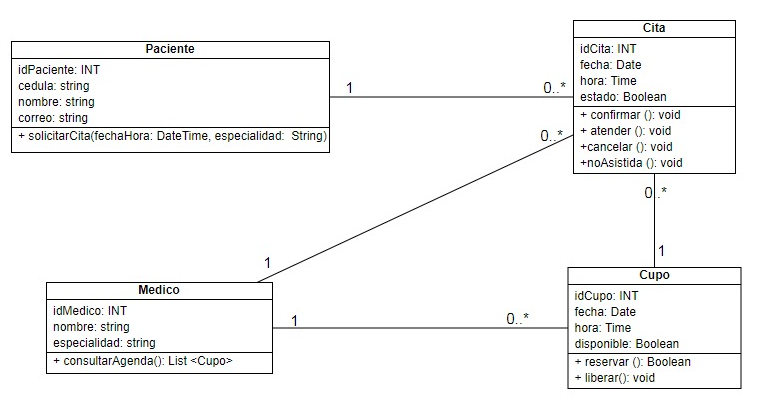
\includegraphics[width=0.85\textwidth]{figuras/clases.png}
\end{center}
\end{tarea}

\begin{tarea}{P2. Modelo funcional --- Diagrama de actividades UML \hfill (8 pts)}
\begin{center}
    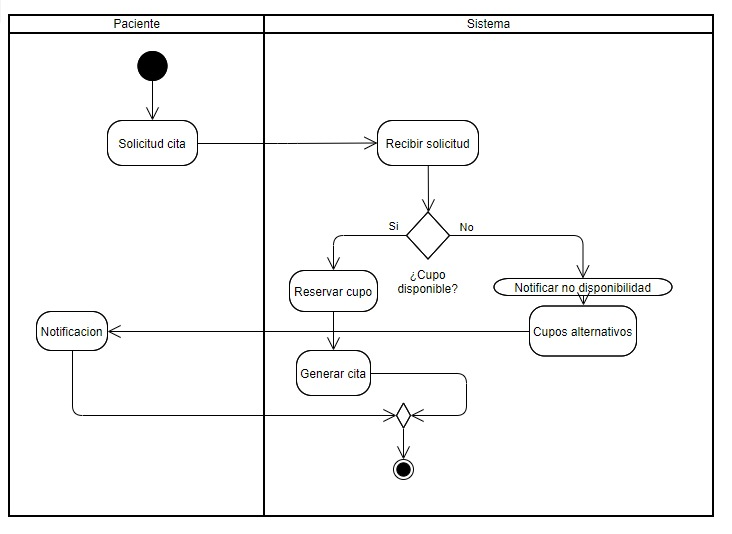
\includegraphics[width=0.85\textwidth]{figuras/actividades.png}
\end{center}
\end{tarea}

\begin{tarea}{P3. Modelo de comportamiento --- M\'aquina de estados UML \hfill (8 pts)}
\begin{center}
    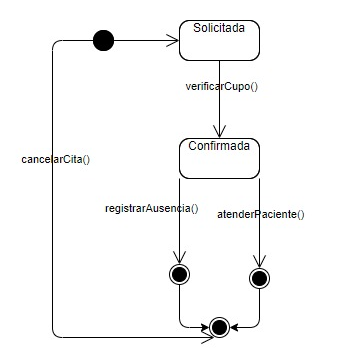
\includegraphics[width=0.85\textwidth]{figuras/estados.png}
\end{center}
\end{tarea}

\begin{tarea}{P4. Consistencia entre las tres perspectivas \hfill (7 pts)}
\small
\begin{tabularx}{\linewidth}{@{}X X X@{}}
    \toprule
    \hd{Evento (P3)} & \hd{Funci\'on/Acci\'on (P2)} & \hd{Entidad/Atributo (P1)}\\
    \midrule
    \texttt{verificarCupo()} [true] & Reservar cupo y confirmar cita & \textsf{Cupo.disponible} (false), \textsf{Cita.estado} (Confirmada)\\
    \rowcolor{rowgray}
    \texttt{verificarCupo()} [false] & Notificar no disponibilidad & Lectura de \textsf{Cupo.disponible}\\
    \texttt{atenderPaciente()} & Registrar atenci\'on & \textsf{Cita.estado} ( Atendida)\\
    \rowcolor{rowgray}
    \texttt{cancelarCita()} & Cancelar reserva & \textsf{Cita.estado}(Cancelada), \textsf{Cupo.disponible} ( true)\\
    \texttt{registrarAusencia()} & Registrar inasistencia & \textsf{Cita.estado} ( No asistida)\\
    \bottomrule
\end{tabularx}

\vspace{3pt}
\textbf{Defecto detectado y correcci\'on:}
\textit{Defecto:} En la versi\'on inicial de P1 no exist\'ia un m\'etodo en la clase \textsf{Cita} para manejar la inasistencia del paciente impulsada por el evento \texttt{registrarAusencia()} de P3.  
\textit{Correcci\'on:} Se actualiz\'o la clase \textsf{Cita} agregando expl\'icitamente la operaci\'on \texttt{marcarNoAsistida(): Void}.
\end{tarea}

\begin{tarea}{P5. Especificaci\'on de requisitos con esquema de atributos \hfill (10 pts)}
\small
\textbf{1. RF-01: Agendamiento y verificacion de cupo}  
\textit{Descripci\'on:} El sistema debe permitir al paciente agendar una cita m\'edica verificando disponibilidad de cupo en la agenda del m\'edico y confirmando de forma autom\'atica.  
\textit{Identificador:} RF-01 | Prioridad: Alta | Estado: Aprobado | Fuente: Cl\'inica (L\'inea 2)| Estabilidad: Alta | Versi\'on: 1.0 | Verificaci\'on: Pruebas de Integraci\'on.

\textbf{2. RF-02: Cancelaci\'on de citas }  
\textit{Descripci\'on:} El sistema debe permitir cancelar una cita confirmada mientras no haya sido atendida previamente. 
\textit{Identificador:} RF-02 | Prioridad: Media | Estado: Aprobado | Fuente: Cl\'inica (L\'inea 6) | Estabilidad: Alta | Versi\'on: 1.0 | Verificaci\'on: Pruebas de sistema.

\textbf{3. RNF-01: Eficiencia de Desempe\~no (Tiempo de Respuesta)}  
\textit{Caracter\'istica ISO 25010:} Eficiencia de desempe\~no / Comportamiento temporal.  
\textit{Descripci\'on:} El sistema debe procesar el agendamiento y confirmaci\'on con rapidez.  
\textit{M\'etrica/Umbral:} Tiempo de respuesta transcurrido $\le 3.0$ segundos bajo una carga de hasta 100 peticiones concurrentes.  
\textit{Identificador:} RNF-01 | Prioridad: Alta | Estado: Aprobado | Fuente: Directriz de negocio (L\'inea 7) | Estabilidad: Media | Versi\'on: 1.0 | Verificaci\'on: Pruebas de Carga.

\textbf{4. RNF-02: Seguridad}  
\textit{Caracter\'istica ISO 25010:} Seguridad / Confidencialidad.  
\textit{Descripci\'on:} El sistema debe proteger los datos personales del paciente cifrando la informaci\'on en reposo y tr\'ansito.  
\textit{M\'etrica/Umbral:} Cifrado AES-256 en BD para atributos sensibles. 
\textit{Identificador:} RNF-02 | Prioridad: Alta | Estado: Aprobado | Fuente: Requisito del sistema (L\'inea 8) | Estabilidad: Alta | Versi\'on: 1.0 | Verificaci\'on: Auditor\'ia de seguridad.
\end{tarea}

\begin{tarea}{P6. Priorizaci\'on MoSCoW \hfill (5 pts)}
\small
\begin{tabularx}{\linewidth}{@{}L{2.0cm} C{2.2cm} X@{}}
    \toprule
    \hd{Requisito} & \hd{MoSCoW} & \hd{Justificaci\'on}\\
    \midrule
    \textbf{RF-01} & \textbf{Must have} & Valor operativo esencial del sistema. Sin agendamiento el software no tiene prop\'osito.\\
    \rowcolor{rowgray}
    \textbf{RNF-02} & \textbf{Must have} & Indispensable por regulaci\'on legal de protecci\'on de datos de salud.\\
    \textbf{RNF-01} & \textbf{Should have} & Importante para la experiencia de usuario, pero no impide el funcionamiento base.\\
    \rowcolor{rowgray}
    \textbf{RF-02} & \textbf{Could have} & Deseable. En un primer MVP las cancelaciones podr\'ian gestionarse administrativamente.\\
    \bottomrule
\end{tabularx}
\end{tarea}

% #####################################################################
\section{Marco normativo de referencia}

Esta prueba operacionaliza las propiedades de calidad de la norma \textit{ISO/IEC/IEEE} 29148:2018 \citep{iso29148_2018} y el modelo de calidad de producto \textit{ISO/IEC} 25010:2023 \citep{iso25010_2023}, junto con las t\'ecnicas de validaci\'on y gesti\'on descritas por Pohl \citep{pohl_2010}, la inspecci\'on formal de Fagan \citep{fagan_1976} y las buenas pr\'acticas recogidas en la gu\'ia SWEBOK v4 \citep{swebok_v4_2024}. Las notaciones de modelado siguen la especificaci\'on \textit{OMG UML} 2.5.1 \citep{omg_uml_2017}.

\vspace{4pt}
\renewcommand{\refname}{Referencias}
\bibliographystyle{plainnat}
\bibliography{referencias}

\end{document}
